\documentclass[twocolumn]{aastex61}
% \documentclass{aastex61}

\newcommand{\radmc}{\texttt{RADMC-3D}}
%\newcommand{\kms}{ \textrm{km s}^{-1} }
\newcommand\kms{\ifmmode{\rm km\thinspace s^{-1}}\else km\thinspace s$^{-1}$\fi}
\newcommand{\todo}[1]{ \textcolor{red}{#1}}
\newcommand{\vt}{ {\bm \theta}}
\newcommand{\msun}{M$_\odot$}
\newcommand{\gw}{GW\,Ori}
\newcommand{\twelve}{CO}
\newcommand{\thirteen}{${}^{13}$CO}
\newcommand{\eighteen}{C${}^{18}$O}

\begin{document}

\title{GW Ori: A Massive Triple System with a Circum-triple Disk, Caught at a Young Age}

\correspondingauthor{Ian Czekala}
\email{iczekala@stanford.edu}

\author[0000-0002-1483-8811]{Ian Czekala} % ORCID ID
\affiliation{Department of Physics and Astronomy,\\
Stanford University, \\
452 Lomita Mall, Stanford, CA 94305 \\}

\author{Sean M. Andrews}
\affiliation{Harvard-Smithsonian Center for Astrophysics, \\
60 Garden Street, Cambridge, MA 02138 \\}

\author{Guillermo Torres}
\affiliation{Harvard-Smithsonian Center for Astrophysics, \\
60 Garden Street, Cambridge, MA 02138 \\}

\author{et al.}

 % E.~L.~N.~Jensen\altaffilmark{2}, K.~G.~Stassun\altaffilmark{3,4}, G.~Torres\altaffilmark{1}, D.~J.~Wilner\altaffilmark{1}, \& Joseph Rodriguez\altaffilmark{2}.}
% \altaffiltext{1}{}
% \altaffiltext{2}{}
% \altaffiltext{3}{Department of Physics and Astronomy, Swarthmore College, 500 College Avenue, Swarthmore, PA 19081}
% \altaffiltext{4}{Department of Physics and Astronomy, Vanderbilt University, Nashville, TN 37235}
% \altaffiltext{5}{Department of Physics, Fisk University, Nashville, TN 37208}

\begin{abstract}
We present spatially and spectrally resolved Atacama Large Millimeter/submillimeter Array (ALMA) observations of gas and dust in the disk orbiting the pre-main sequence triple GW Ori. We forward-model the \thirteen\ and \eighteen\ $J$=2--1 transitions to put precise constraint on the total stellar mass of $5.5 \pm 0.2\,M_\odot$. We use 35 years of radial velocity monitoring to update the orbital solution and place constraints on the orbital parameters of the secondary and tertiary components. Combining the measurements from these two datasets yields a precise constraint on the primary stellar mass of $M_A = 4.4\pm 0.18\,M_\odot$. We show that this precise mass is consistent with the predictions of leading pre-main sequence evolutionary models based upon its observed photospheric properties and suggests that \gw\ system is caught at a very young (and rare) evolutionary state for an intermediate mass star, less than 1~Myr. We put constraints on the orbital configuration of the triple system within the massive disk and discuss this in the context of star and planet formation.
\end{abstract}
\keywords{ protoplanetary disks -- stars: fundamental parameters -- stars: pre-main sequence -- stars: individual (GW Ori)}

\section{Introduction} \label{sec:intro}

Pre-main sequence stars in multiple systems--for which it is possible to precisely measure their fundamental stellar properties--can serve as touchstones for understanding the final stages of stellar formation and the conditions under which planetary systems are assembled. While recent decades have seen steady progress in understanding binary formation in general, lingering uncertainties still remain about the characteristics of young close-in spectroscopic binaries and higher order systems \citep{duchene13}.

\gw\ was one of the first T Tauri stars to be revealed as a single-lined spectroscopic binary \citep{mathieu91}, with a composite spectral type of late G and an orbital period of 240 days. Long term radial velocity monitoring hinted at the presence of a third body in the system with a period of $\sim$$10\,$ years, and was subsequently confirmed by infrared interferometry \citep{berger11}. Despite concerted efforts, there have not been any detections of the spectroscopic lines from the secondary or tertiary stars in optical spectra to date, suggesting a large flux contrast between A and the other components of the system. \gw\ is a member of the $\lambda$ Orionis star forming complex, a young OB association \citep{dolan00,dolan01,dolan02} in Orion. The most recent and precise measurements of the distance to Orion Nebula Complex is a VLBA parallax measurement of $388\pm5\,$pc \citep{kounkel16}, which we adopt as the distance to \gw.

A reservoir of circumstellar material orbiting \gw\ was inferred from near and far-infrared emission in excess of the stellar photosphere \citep{mathieu91}, and was subsequently confirmed by a strong single-dish sub-millimeter detection of the dust continuum, suggesting a massive circumstellar disk \citep[$M_\mathrm{disk} \gtrsim 0.1\,M_\odot$;][]{mathieu95}. Quasi-periodic photometric dimminings of \gw\ have been observed to occur on $\sim100\,$ day timescales, and are suspected to be due from material in the circumstellar disk occulting the primary star \citep{shevchenko92,shevchenko98}, although the fact that edge-on orbital inclinations are ruled out complicates this interpretation. \todo{correspond with Joey about KELT dimmings}.

Mid-infrared spectroscopic observations of \gw\ detected CO fundamental emission with line profiles that have both a narrow and broad component, requiring a complicated emission region and temperature structure in the inner disk \citep{najita03}. \citet{fang14} compile several epochs of spectral energy distributions (SEDs) spanning decades and find that the mid-infrared emission is variable on the timescale of years. The SED and its variability can be explained by a gapped disk with changes in the structure of the inner disk.
% There is a paper about \ion{Mg}{2} observations from IUE and HST on GW Ori, which include it as part of a survey. I'm not sure if there is much we say about it in this introduction, other than there is a warm wind at several AU. \citep{lopez-martinez15}.


% \todo{{\it circle back to big picture/context}}: why GW Ori is interesting in the larger astrophysics landscape.  probably most interesting to mention here the nominal masses are large, and so its like a super-young version of Max Moe's multiple systems (possible SNe progenitors?).  also interesting from the perspective of forming high-order multiples (compact triple system).  finally note that its a particularly interesting test of pre-main sequence models at the high mass end of the IMF.  explain that its useful to get a mass measurement and why.

Orbital constraints from radial velocity \citep{mathieu91,fang14} and astrometric \citep{berger11} monitoring imply that the \gw\ system is massive ($M_\mathrm{tot} > 5\,M_\odot$), with A being the dominant component ($M_A > 3\, M_\odot$). Such a large mass with only a late G spectral type implies that \gw\ A (and the system) must be very young according to models of pre-main sequence stellar evolution ($< 1$\,Myr).

When it reaches the main sequence in $\sim$$10\,$ Myr, \gw\ A will have a B spectral type. B star lifetimes are notoriously short--this means that the current state of \gw\ represents an interesting if brief snapshot of the evolutionary history of high mass stars. Interestingly, \gw\ might represent a younger analogue to the new class of binaries recently discovered by \citet{moe15}, which are comprised of a main sequence B star with a pre-main sequence T~Tauri star companion. Refining the stellar properties of the \gw\ system will enable important tests of our understanding of pre-main sequence evolutionary models at the high mass end of the initial mass function.

% \todo{{\it paper overview}}: one sentence reminding people that we can use the disk to get the mass (cite our previous papers).  what data we have for GW Ori and what we will do with it here.  section breakdowns.

Spatially and spectrally resolved sub-millimeter observations of molecular gas lines in protoplanetary disks can be used to reconstruct the disk velocity field and independently measure the total stellar mass of the system \citep[e.g.,][]{rosenfeld12b,czekala15a,czekala16}. Here we report the first resolved sub-mm observations of the \gw\ system with the ALMA interferometer, which reveal the presence of a large and massive protoplanetary disk. We forward-model the protoplanetary disk to infer the total mass of the enclosed stars. We also re-analyze 35 years of optical spectra to derive updated orbital constraints on \gw\ A, B, and C. We combine these mass constraints with measurements of the photospheric properties of A to evaluate its agreement with leading pre-main sequence models. We also discuss the structure and orientation of the protoplanetary disk with respect to the putative orbital inclinations of the stellar components and place the quasi-period eclipsing nature of \gw\ in the context of other recently discovered ``dipper'' stars \citep[e.g.,][]{ansdell16b,ansdell16a}.

\section{Observations and Data Reduction \label{sec:obs}}


\subsection{Millimeter Interferometry}

\begin{figure*}[ht!]
\begin{center}
  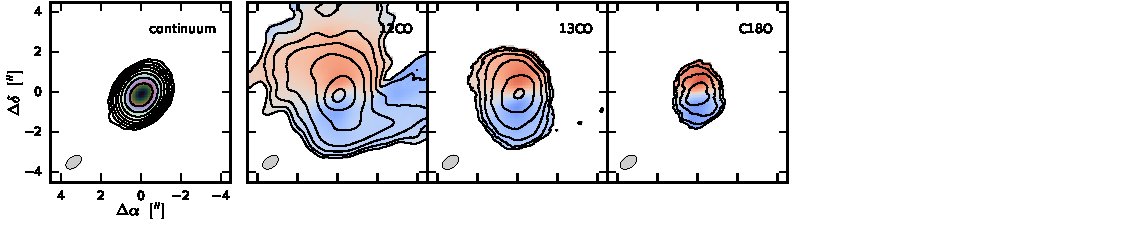
\includegraphics[width=\linewidth]{moments.pdf}
  \figcaption{({\it left}) A 226\,GHz continuum image.  Contours start at 5$\times$ the RMS noise level and increase by factors of 2.  The synthesized beam geometry is shown in the lower left corner.  ({\it middle, left to right}) Maps of the $^{12}$CO, $^{13}$CO, and C$^{18}$O velocity-integrated intensities (contours, starting at 10, 3, and 3$\times$ the RMS noise levels, respectively, and increasing by factors of 2) overlaid on the intesity-weighted projected velocities (color-scale).  Note the prominent molecular cloud contamination in the $^{12}$CO map (see also Fig.~\ref{fig:chanmaps}).  ({\it right}) Spatially integrated spectra (inside the same {\tt CLEAN} mask, and smoothed with an 0.85\,km\,s$^{-1}$ Hanning kernel) for each CO line.
  \label{fig:moments}}
  \end{center}
\end{figure*}

GW Ori was observed with the ALMA interferometer on 2015 May 14 (program ID 2012.1.00496.S), with 37 of the 12\,m main array antennas configured to span baselines of 23--558\,m.  The double sideband Band 6 receivers were employed in dual polarization mode, and the ALMA correlator was set up to process data in 4 spectral windows (SPWs).  Two of these SPWs, centered at 220.426 and 230.450\,GHz to observe the nearby $^{13}$CO and $^{12}$CO $J$=2--1 transitions (at rest frequencies of 220.399 and 230.538\,GHz, respectively), covered 234\,MHz of bandwidth in 3840 channels (a 61\,kHz channel spacing).  One other sampled 469\,MHz around 219.763\,GHz to observe the nearby C$^{18}$O $J$=2--1 transition (at rest frequency 219.560\,GHz) with 3840 channels (a 122\,kHz channel spacing).  The last SPW sampled the continuum in a 1.875\,GHz range around 231.956\,GHz using 128 coarse channels (a 15.625\,MHz channel spacing).

The observations cycled between GW Ori and the quasar J0510+1800 with a 7 minute cadence.  The quasar J0423-0120 and Ganymede were observed as bandpass and flux calibration sources, respectively, at the start of the execution block.  The total on-source integration time for GW Ori was 16 minutes.  The observing conditions were typical for Band 6 projects, with a precipitable water vapor level around 1.1\,mm.

The visibility data were calibrated with standard procedures using the {\sc CASA} software package (v4.4).  The raw, observed visibility phases were adjusted based on the contemporaneous measurements of water vapor radiometers, flagged when applicable, and then the bandpass shape in (and between) each SPW was calibrated based on the observations of J0423-0120.  The absolute amplitude scale was determined based on the observations of Ganymede.  The complex gain behavior of the array and atmosphere was corrected based on the repeated observations of J0510+1800.  The calibrated visibilities showed a strong continuum signal, suggesting that self-calibration could significantly improve the data quality.  An initial model based on a preliminary continuum image was used for two rounds of phase-only self-calibration (on 30\,s, then 6\,s intervals) and one additional round that included the amplitudes (on a 7 minute scan interval).  This self-calibration reduced the RMS noise level in the continuum by a factor of $\sim$40.  After applying the self-calibration tables to the entire dataset (channel by channel),  we parsed out data products for each individual emission tracer of interest.  A set of continuum visibilities was constructed by spectrally averaging the line-free channels in each SPW into $\sim$125\,MHz increments.  The spectral visibilities for the $^{12}$CO, $^{13}$CO, and C$^{18}$O lines were continuum-subtracted and regridded into 170\,m s$^{-1}$-wide channels in the LSRK restframe over a $\sim$10\,km s$^{-1}$ range around the line centers.

These fully reduced visibility sets were then imaged by Fourier inversion assuming a Briggs (robust=0.5) weighting scheme and deconvolution with the standard {\tt CLEAN} algorithm.  Some basic image properties for the synthesized continuum image and spectral line image cubes are listed in Table~\ref{tab:ims}.  The continuum and spectral line moment maps are shown together in Figure~\ref{fig:moments}, along with a comparison of the integrated spectra.  The channel maps for individual lines are compiled in Figure~\ref{fig:chanmaps}.

\begin{deluxetable}{lcc}[b!]
\tablewidth{18pc}
\tablecaption{ALMA Image Properties  \label{tab:ims}}
\tablehead{
\colhead{} &
\colhead{} &
\colhead{RMS}
\\
\colhead{} &
\colhead{beam dimensions} &
\colhead{mJy beam$^{-1}$}}
\startdata
226\,GHz continuum  & $0\farcs88\times0\farcs54$, 126\degr\ & 0.055 \\
$^{12}$CO $J$=2$-$1 & $0\farcs89\times0\farcs56$, 126\degr\ & 6     \\
$^{13}$CO $J$=2$-$1 & $0\farcs93\times0\farcs59$, 126\degr\ & 8     \\
C$^{18}$O $J$=2$-$1 & $0\farcs92\times0\farcs58$, 126\degr\ & 5     \\
\enddata
\tablecomments{The RMS noise levels recorded for the spectral line cubes correspond to the values per 170\,m s$^{-1}$ channel.}
\end{deluxetable}

\begin{figure*}[ht!]
\begin{center}
  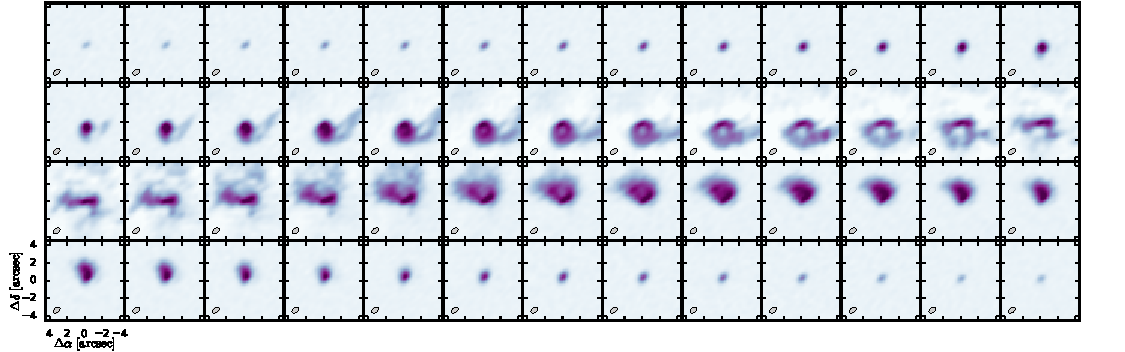
\includegraphics[width=\linewidth]{chanmaps_12co.pdf}
  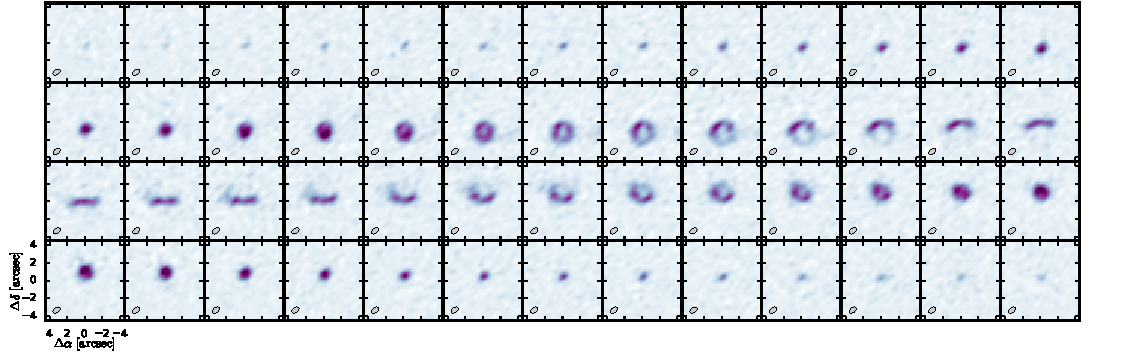
\includegraphics[width=\linewidth]{chanmaps_13co.pdf}
  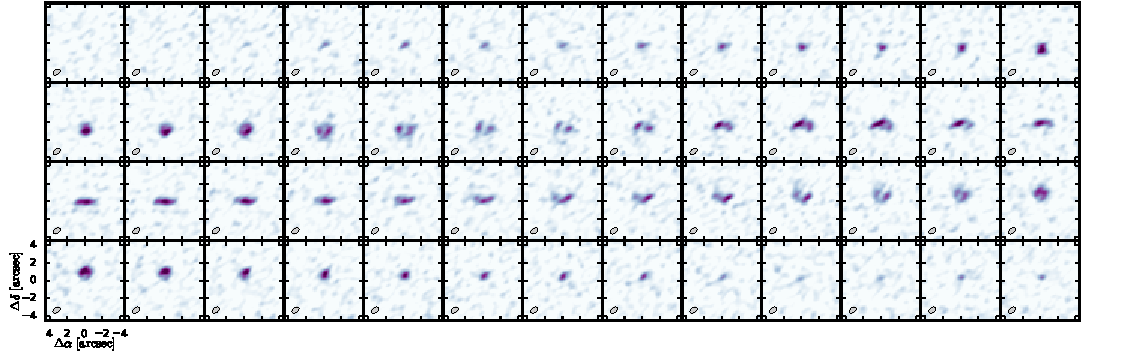
\includegraphics[width=\linewidth]{chanmaps_c18o.pdf}
  \figcaption{Channel maps of the $^{12}$CO, $^{13}$CO, and C$^{18}$O ({\it from top to bottom}) line emission from the GW Ori disk.  Each channel represents the emission in a 170\,m\,s$^{-1}$-wide velocity bin.  LSRK velocities are indicated in the upper left, and synthesized beam sizes in the lower left, or each panel.  Scale bars are provided at the bottom right of each set of channel maps.
  \label{fig:chanmaps}}
  \end{center}
\end{figure*}

The 226\,GHz (1.3\,mm) continuum map shows a bright (flux density = 202\,mJy), compact but marginally resolved (deconvolved Gaussian FWHM $\approx 0\farcs9$) source centered on the GW Ori stellar system, with a peak intensity of 67\,mJy beam$^{-1}$ (S/N $\approx 1200$).  A crude estimate of the emission geometry (from a Gaussian fit to the visibilities) suggests an inclination of 35--40\degr\ from face-on, with the major axis oriented $\sim$170\degr\ E of N.

The CO isotopologue channel maps reveal bright (integrated intensities of 41.8, 5.7, and 0.8\,Jy\,km\,s$^{-1}$ for $^{12}$CO, $^{13}$CO, and C$^{18}$O, respectively) and extended (FWHM $\sim 2\farcs5$) emission that is clearly in rotation around the continuum centroid, spanning a projected velocity range of $\pm$5\,km s$^{-1}$ from the line center.  The line emission is blueshifted to the south and redshifted to the north, consistent with the orientation estimated from the continuum emission.  The peak intensities for each line are $\sim$800, 290, and 55\,mJy beam$^{-1}$ in the brightest channels (peak S/N $\approx 130$, 35, and 14) for $^{12}$CO, $^{13}$CO, and C$^{18}$O, respectively.  The $^{12}$CO channel maps show some clear evidence for structured contamination from the surrounding molecular cloud, particularly as a streamer to the west at LSRK velocities $\sim$11--13\,km s$^{-1}$ and some diffuse clumps to the north around 13--14\,km s$^{-1}$.  Those features are much fainter, but still present, in $^{13}$CO emission; they are not apparent in the C$^{18}$O maps.



%begin{figure*}[htb]
%\begin{center}
%  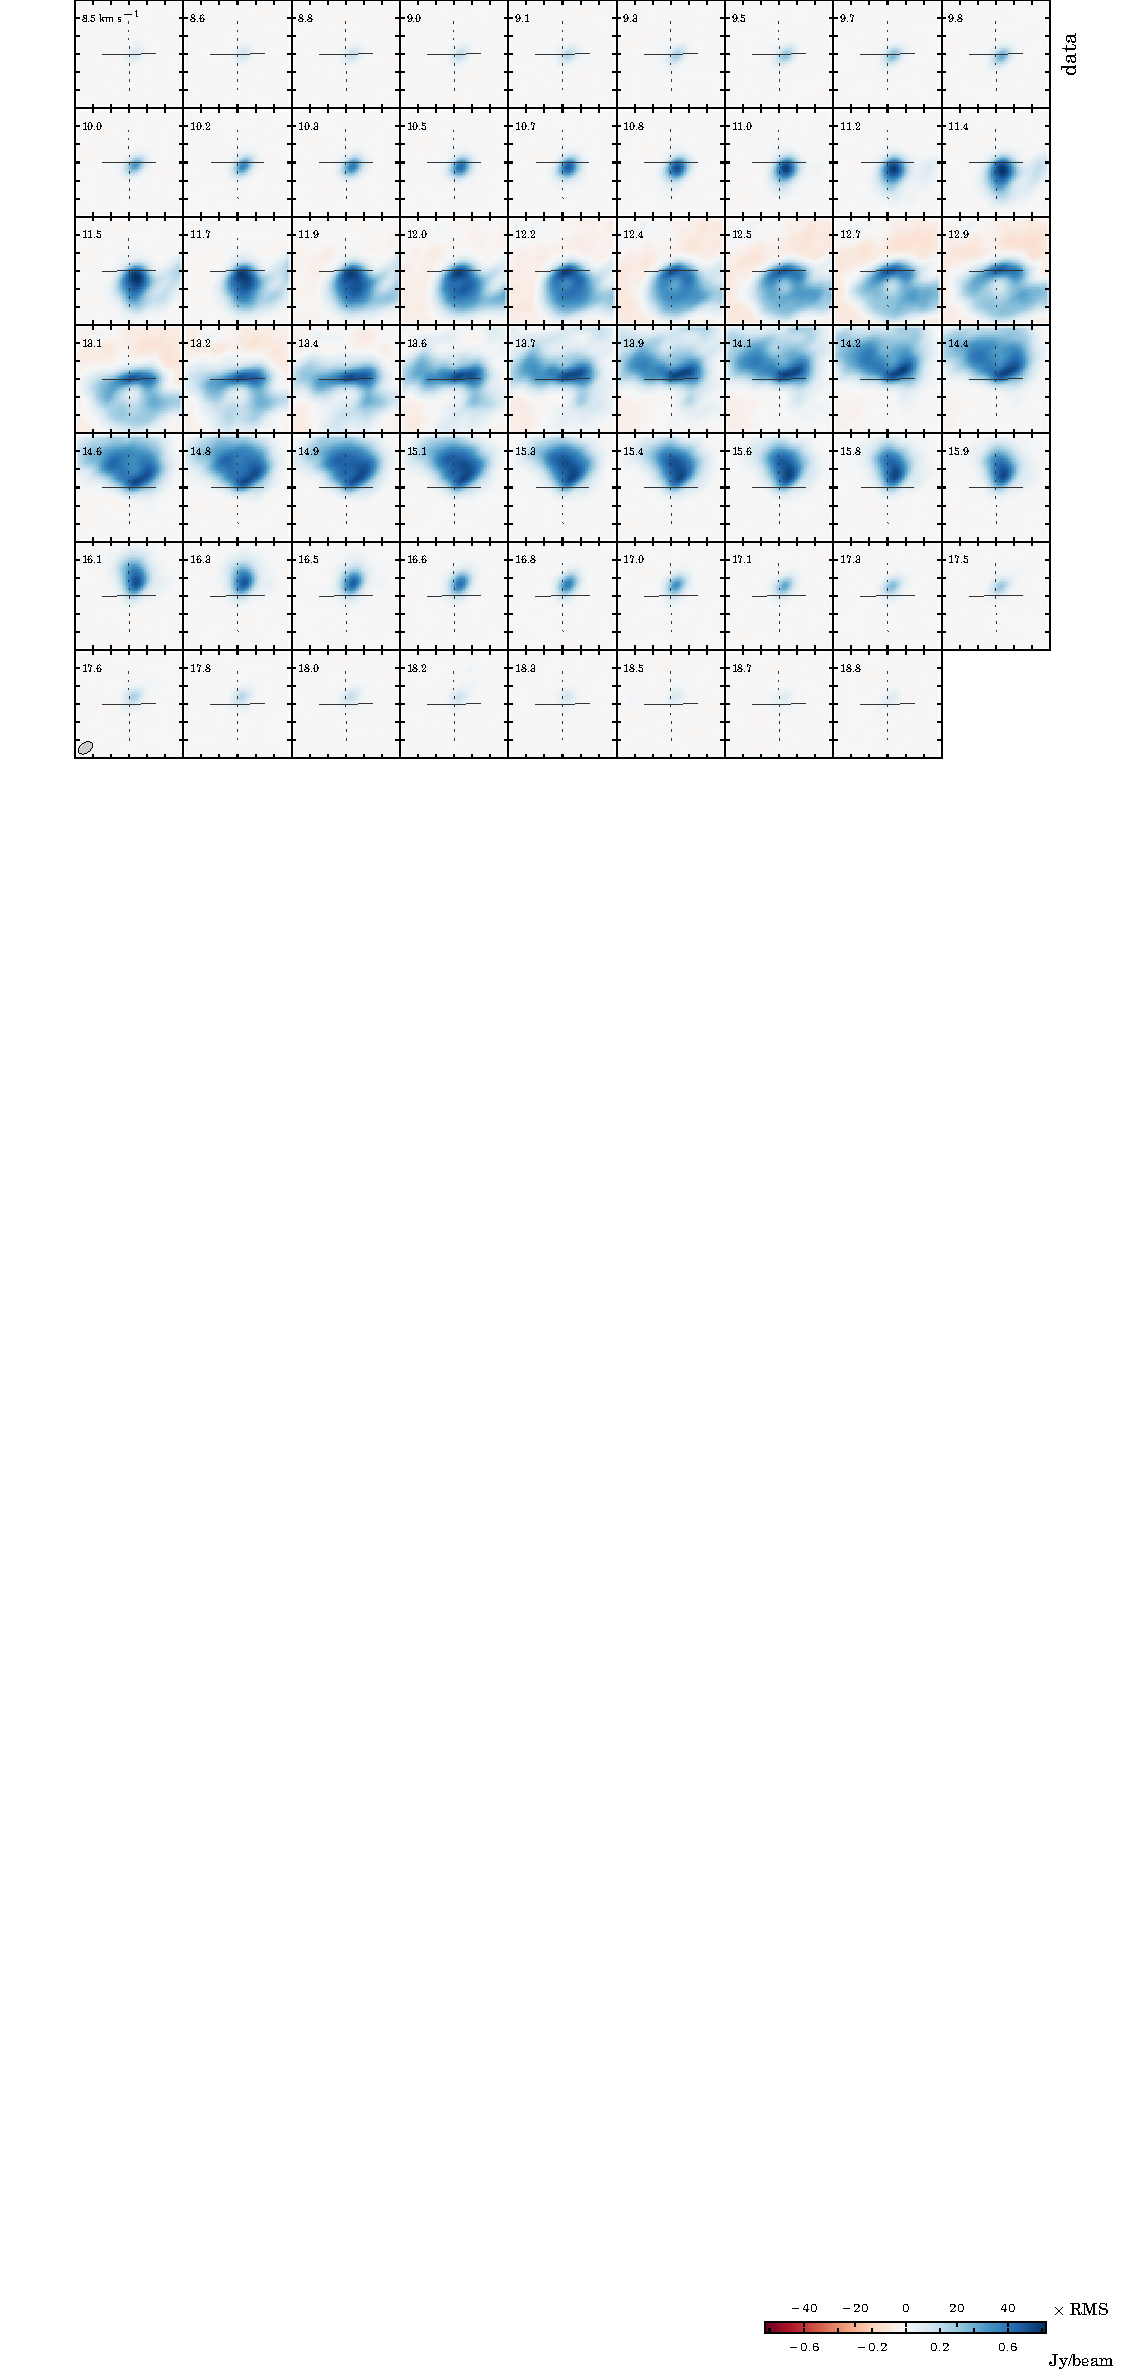
\includegraphics{chmaps_CO.pdf}
%  \figcaption{\twelve\ channel maps. Due to the nearby cloud contamination, we do not model these. (Or, we model only the XX channels.)
%  \label{fig:chmaps_CO}}
%  \end{center}
%\end{figure*}

%\begin{figure*}[htb]
%\begin{center}
%  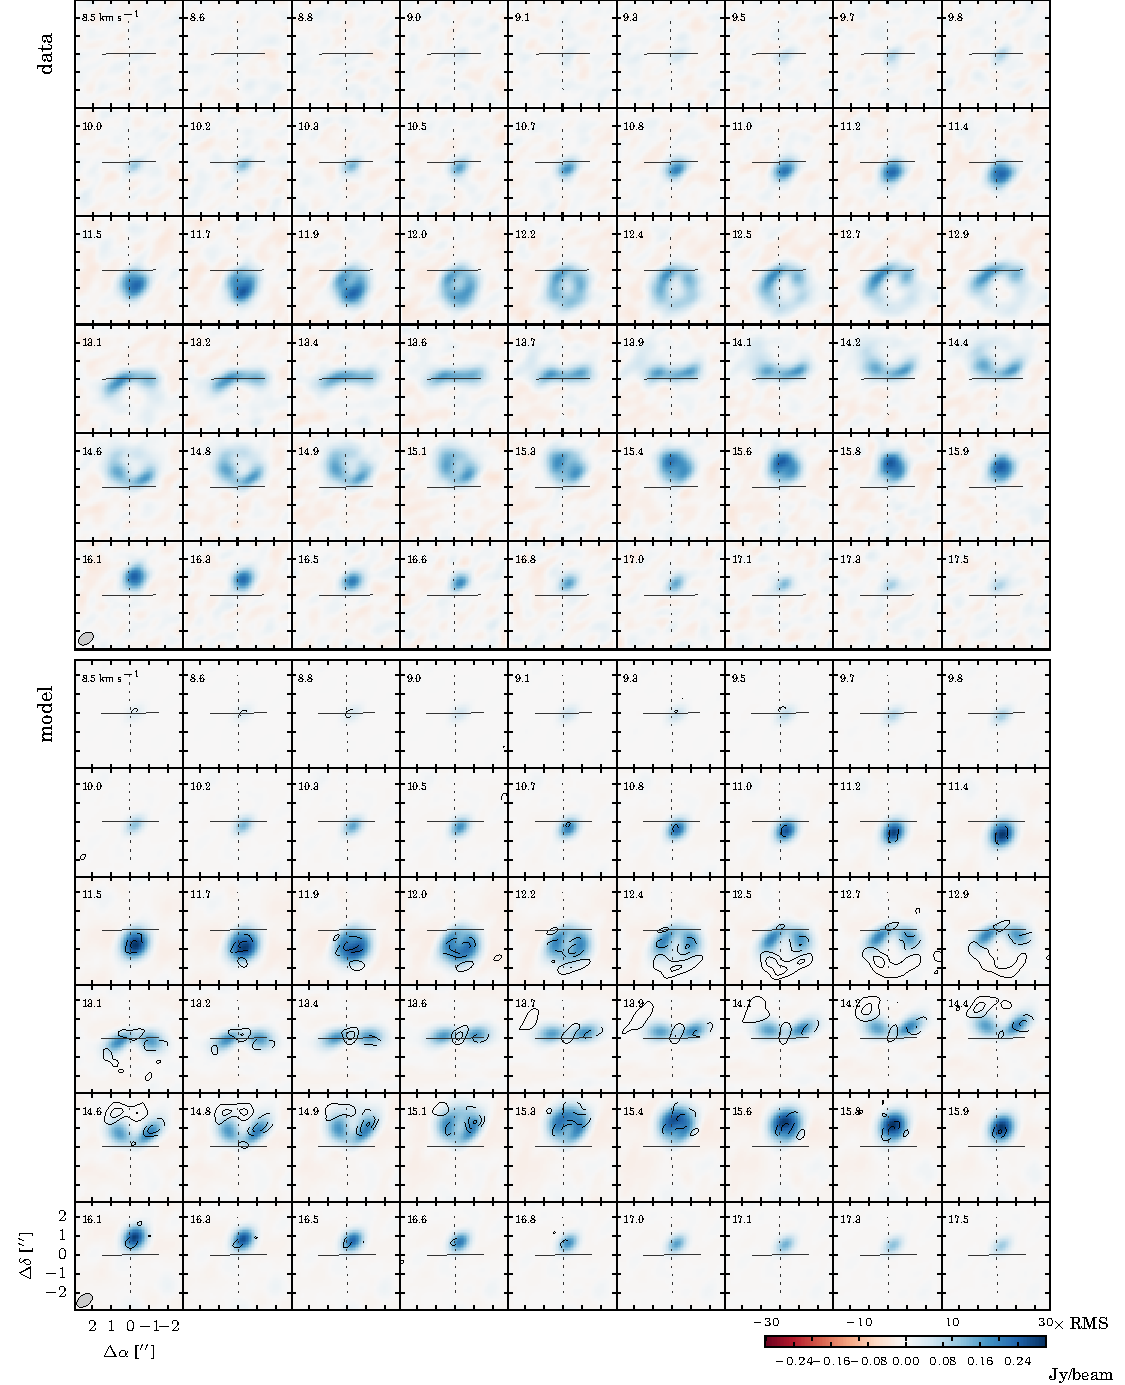
\includegraphics{chmaps_13CO.pdf}
%  \figcaption{\thirteen\ channel maps, model, and residuals.
%  \label{fig:chmaps_13CO}}
%  \end{center}
%\end{figure*}

%\begin{figure*}[htb]
%\begin{center}
%  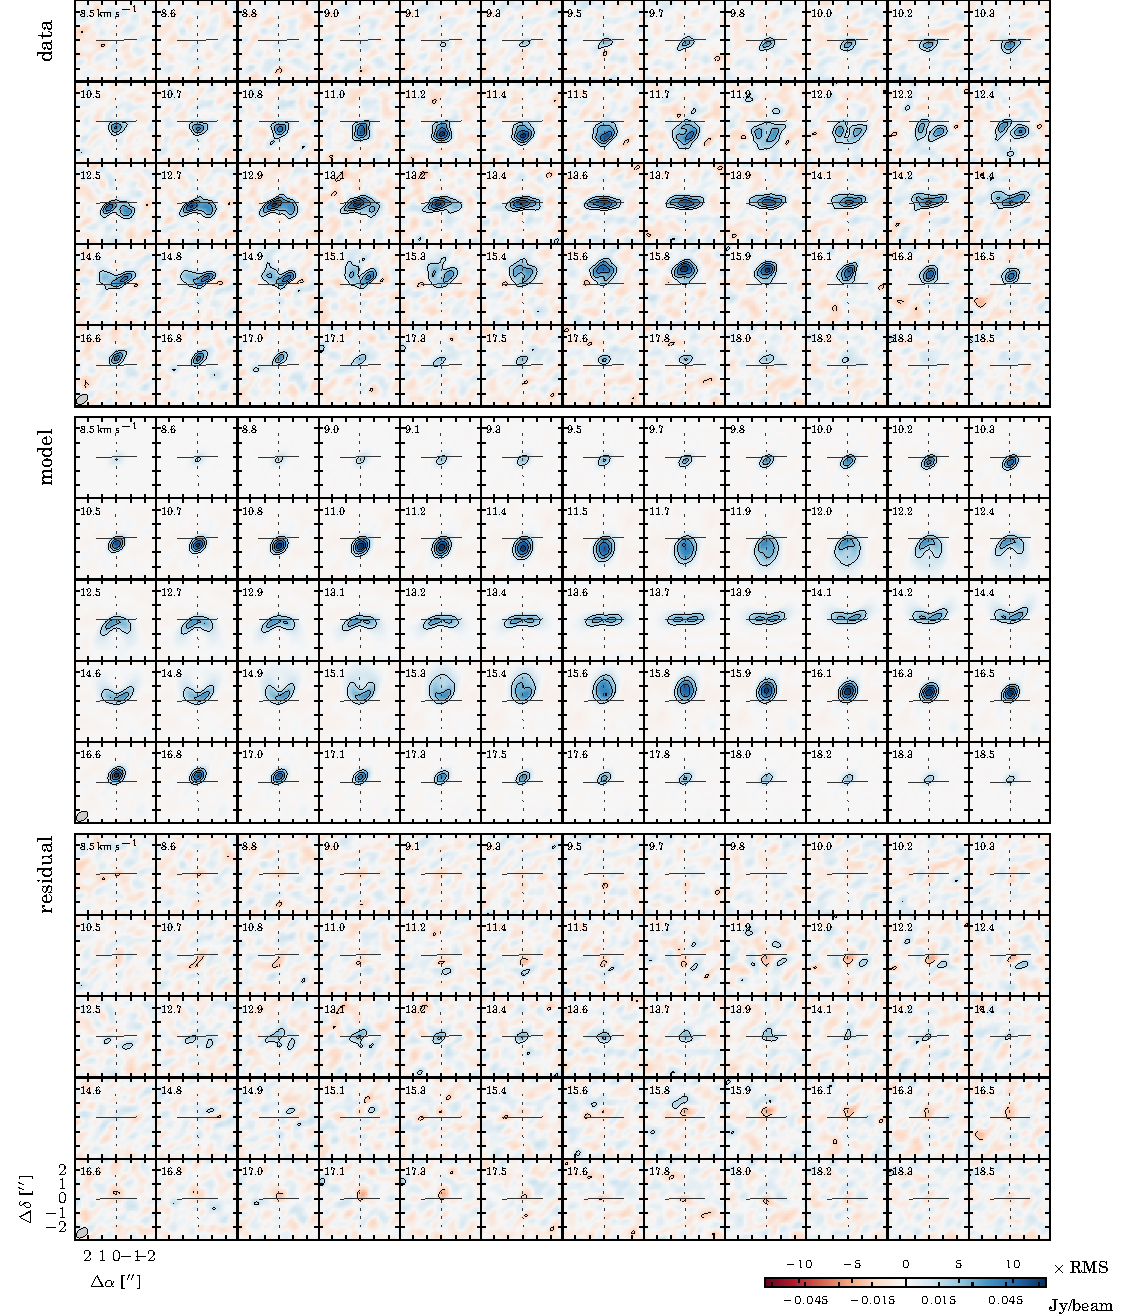
\includegraphics{chmaps_C18O.pdf}
%  \figcaption{\eighteen\ channel maps, model, and residuals.
%  \label{fig:chmaps_C18O}}
%  \end{center}
%\end{figure*}



\subsection{Optical Spectroscopy \label{sec:spectroscopy}}

\gw\ was monitored spectroscopically at the Harvard-Smithsonian Center for Astrophysics for more than 35 years, beginning in 1981 November. A total of 208 spectra were gathered through 2009 April using three nearly identical echelle spectrographs (Digital Speedometers, DS; now decommissioned) with a resolving power of $R \approx 35,000$ mounted on three different telescopes: the 1.5m Tillinghast reflector at the Fred L.\ Whipple Observatory (Mount Hopkins, AZ), the 4.5m-equivalent Multiple Mirror Telescope (also on Mount Hopkins) before conversion to a monolithic mirror, and occasionally also on the 1.5m Wyeth reflector at the Oak Ridge Observatory (in the town of Harvard, MA).  Each instrument was equipped with an intensified photon-counting Reticon detector limiting the output to a single echelle order 45~\AA\ wide, which was centered on the region of the \ion{Mg}{1}\,b triplet at 5187~\AA\ \citep[see][]{latham92}. The signal-to-noise ratios of these observations range from 14 to 59 per resolution element of 8.5~\kms. Wavelength calibrations were based on exposures of a Thorium-Argon lamp taken before and after each science exposure. Reductions were performed with a dedicated pipeline, and the zero-point of the velocities was monitored regularly by means of exposures of the evening and morning twilight sky. A further 80 spectra of \gw\ were collected with the Tillinghast Reflector Echelle Spectrograph \citep[TRES;][]{furesz08}, a bench-mounted, fiber-fed echelle instrument mounted on the 1.5m Tillinghast reflector with a resolving power of $R \approx 44,000$ and delivering 51 orders covering the wavelength interval 3900--9100~\AA. These observations were made between 2010 November and 2016 April.  Signal-to-noise ratios at 5200~\AA\ range from 28 to 195 per resolution element of 6.8~\kms. Wavelength calibration was carried out as above, and reductions were performed as described by \cite{buchhave10}. Radial-velocity standard stars were observed each night to monitor the zero point and place it on the same system as the DS observations to within $\sim$0.1~\kms.

All of our spectra appear single-lined.  Radial velocities were measured by cross-correlation using the IRAF\footnote{IRAF is distributed by the National Optical Astronomy Observatories, which are operated by the Association of Universities for Research in Astronomy, Inc., under cooperative agreement with the National Science Foundation.} task {\tt XCSAO} \citep{kurtz98}, with templates taken from a large library of calculated spectra based on model atmospheres by R.\ L.\ Kurucz \citep[see][]{nordstroem94,latham02}. These synthetic templates cover a 300~\AA\ region centered on the \ion{Mg}{1}\,b triplet, and are available for a wide range of effective temperatures ($T_{\rm eff}$), surface gravities ($\log g$), metallicities ([Fe/H]), and rotational broadenings ($v \sin i$ when seen in projection). The optimal template was selected by running grids of cross-correlations over broad ranges in the template parameters, as described by \cite{torres02}, seeking the best match as measured by the peak cross-correlation coefficient averaged over all exposures. This was done separately for the DS and TRES spectra, using only the order centered on the \ion{Mg}{1}\,b line, for consistency.

In principle these template parameters may be interpreted as estimates of the physical properties of the star. In practice, however, the narrow wavelength range ($\sim$100~\AA\ for TRES, 45~\AA\ for DS) limits the analysis by introducing a degeneracy between temperature, surface gravity, and metallicity such that a match of nearly equal quality is obtained by slightly increasing or decreasing these template parameters in tandem. We therefore made the reasonable assumption that \gw\ has solar metallicity, as expected for young stars, and we held $\log g$ fixed at a range of values between 2.5 and 4.0, varied in steps of 0.5, and solved only for $T_{\rm eff}$ and $v \sin i$. The best fit was found for $\log g = 3.0$, for both the DS and TRES spectra, and the resulting temperatures and rotational broadenings were very similar: 5180~K and 43~\kms\ for DS, and 5210~K and 44~\kms\ for TRES. For the remainder of the paper we adopt consensus values of $T_{\rm eff} = 5200 \pm 200$~K and $v \sin i = 44 \pm 2~\kms$. Because of the strong dependence of temperature on the adopted surface gravity (and metallicity) we cannot rule out a bias in $T_{\rm eff}$, which may also have a contribution from veiling (not considered in our templates), if significant in the spectral region analyzed.  Radial velocities were based on a template with parameters nearest to those reported above ($T_{\rm eff} = 5250$~K, $v \sin i = 40~\kms$, $\log g = 3.0$); they are listed in Table~\ref{tab:RVs} in the heliocentric frame along with our uncertainty estimates from {\tt XCSAO}. The average internal errors for the DS and TRES velocities are 1.41 and 0.98~\kms, respectively.

\begin{deluxetable}{lcccc}
\tablewidth{18pc}
\tablecaption{Heliocentric radial velocity measurements of \gw.
\label{tab:RVs}}
\tablehead{
\colhead{HJD} &
\colhead{RV} &
\colhead{$\sigma_{\rm RV}$} &
\colhead{} &
\colhead{}
\\
\colhead{(2,400,000$+$)} &
\colhead{(\kms)} &
\colhead{(\kms)} &
\colhead{$\phi_{\rm in}$} &
\colhead{$\phi_{\rm out}$}}
\startdata
    44919.0042 &  31.43  &   1.88   &   0.2480  &  0.9360 \\
    45301.8865 &  26.55  &   1.28   &   0.8338  &  0.0274 \\
    45336.7941 &  24.43  &   1.26   &   0.9784  &  0.0358 \\
    45708.7038 &  30.41  &   1.79   &   0.5187  &  0.1246 \\
    45709.6058 &  35.22  &   1.14   &   0.5225  &  0.1248 \\
\enddata
\tablecomments{Observations up to HJD 2,454,926.6573 were obtained
  with the DS, and the remainder with TRES. Phases in the inner and
  outer orbits are represented with $\phi_{\rm in}$ and $\phi_{\rm
    out}$. This table is available in its entirety in machine-readable
  form.}
\end{deluxetable}


% \subsection{Photometric Observations}
% \textbf{To be included? Joey?}
% Photometry from Grankin, KELT.



\section{Analysis and Results}

\subsection{A Reconstruction of the Disk Velocity Field}
We use the spatially and spectrally resolved molecular line emission observed with ALMA to tomographically model the disk velocity field and make a dynamical measurement of the system mass.  To do that, we follow the forward modeling procedures -- with some modifications as highlighted below -- described in detail by \citet{czekala15a,czekala16}, using the associated open-source software package {\tt DiskJockey}.\footnote{Available under an MIT license at \url{https://github.com/iancze/DiskJockey}.}

\begin{figure*}[ht!]
\begin{center}
  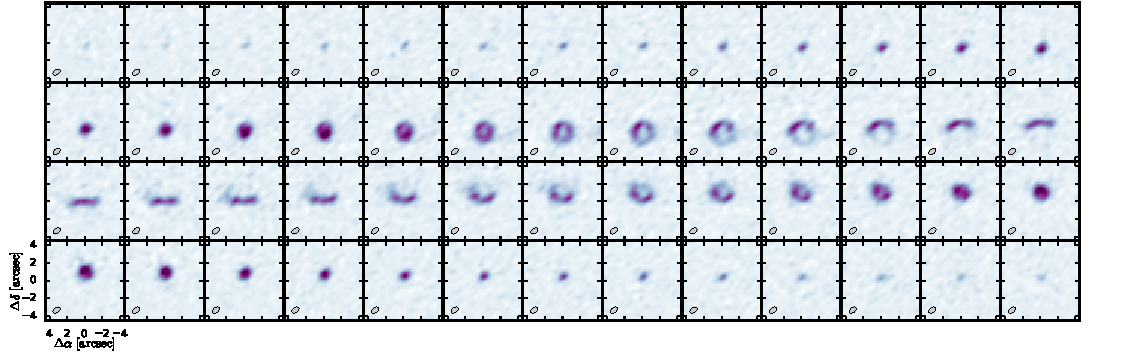
\includegraphics[width=\linewidth]{chanmaps_13co.pdf}
  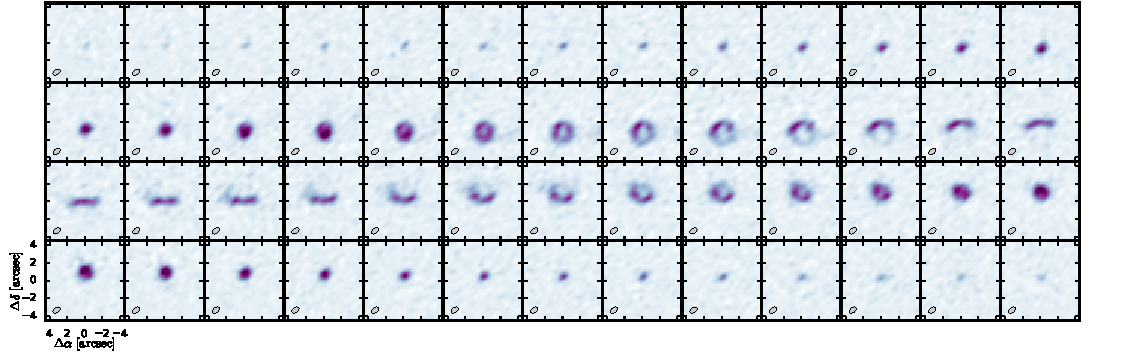
\includegraphics[width=\linewidth]{chanmaps_13co.pdf}
  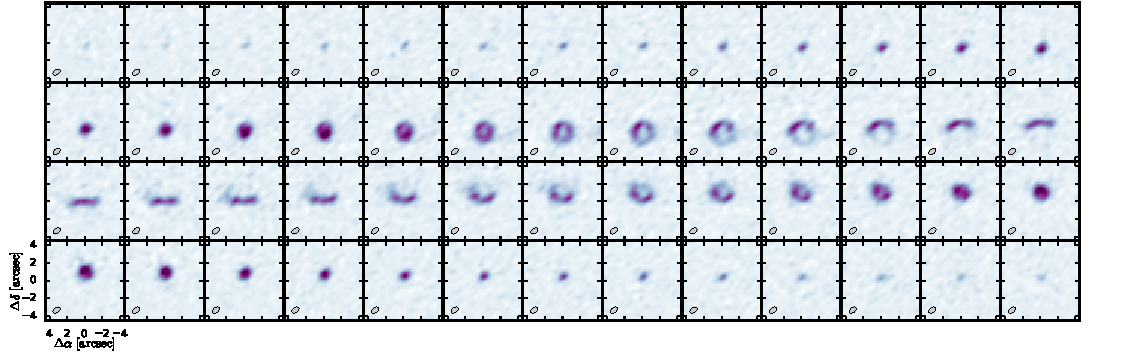
\includegraphics[width=\linewidth]{chanmaps_13co.pdf}
  \figcaption{A comparison of the observed channel maps of the $^{13}$CO line emission ({\it top}) with a ``best-fit" model ({\it middle}; constructed from a synthetic visibility set based on the inferred parameters listed in Table~\ref{table:components} and then imaged in the same way as the data) and the associated residuals ({\it bottom}; the imaged data$-$model residual visibilities).  The annotation is the same as in Fig.~\ref{fig:chanmaps}.
  \label{fig:13co}}
  \end{center}
\end{figure*}

The basis of the parametric physical model adopted in this approach is a radial surface density profile, $\Sigma(r)$, designed to mimic a simple theoretical description for a viscous accretion disk \citep{lyndenbell74,hartmann98}.  It decreases like $1/r$ interior to a characteristic radius $R_c$, and has an exponential taper $e^{-r/R_c}$ at larger radii.  The vertical distribution ($z$-direction) of these densities is controlled by the disk temperatures.  In this study, we generalize the previous {\tt DiskJockey} code to accommodate models with a vertical temperature gradient in order to better account for the observed emission in high quality ALMA datasets.  We follow the standard prescription in the literature \citep{dartois03,andrews12,rosenfeld13a} and define
\begin{equation}
	T(r, z) = T_m + (T_a - T_m)  \sin \left [ \frac{\pi z}{8 H} \right ]^4,
\end{equation}
where $T_m$ and $T_a$ are the midplane and ``atmosphere" radial temperature profiles, presumed to be power-laws with independent normalizations ($T_{m,0}$, $T_{a,0}$) and indices ($q_m$, $q_a$), and $H$ is the scale height calculated for $T_m$.  The density structure, $\rho(r, z)$, is determined by numerically integrating the hydrostatic equilibrium condition for this $T(r,z)$ structure at each radius (normalized by $\Sigma$).

\begin{figure*}[ht!]
\begin{center}
  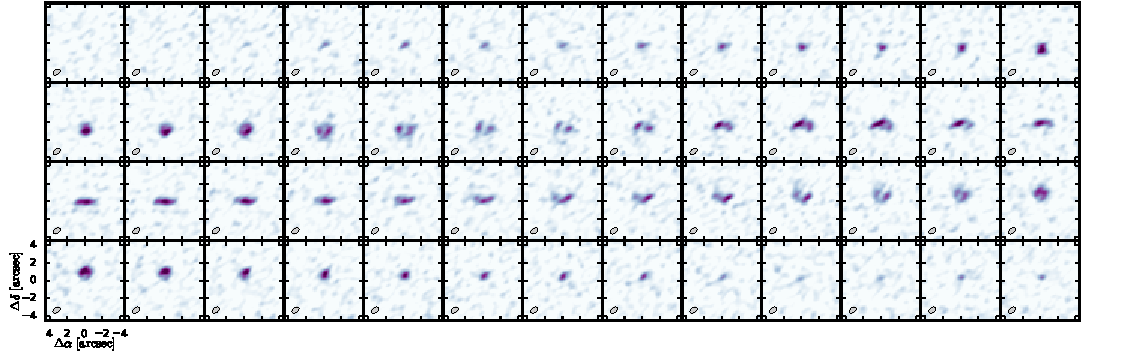
\includegraphics[width=\linewidth]{chanmaps_c18o.pdf}
  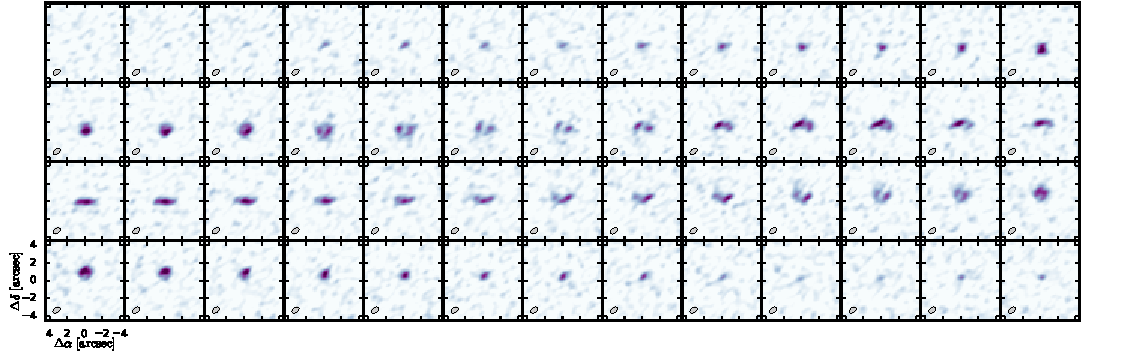
\includegraphics[width=\linewidth]{chanmaps_c18o.pdf}
  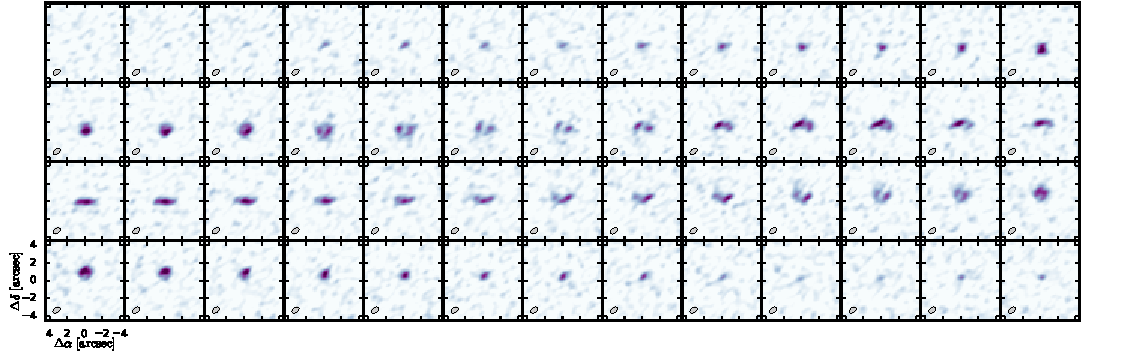
\includegraphics[width=\linewidth]{chanmaps_c18o.pdf}
  \figcaption{A comparison of the observed channel maps of the C$^{18}$O line emission ({\it top}) with a ``best-fit" model ({\it middle}; constructed from a synthetic visibility set based on the inferred parameters listed in Table~\ref{table:components} and then imaged in the same way as the data) and the associated residuals ({\it bottom}; the imaged data$-$model residual visibilities).  The annotation is the same as in Fig.~\ref{fig:chanmaps}.
  \label{fig:c18o}}
  \end{center}
\end{figure*}


To convert the total gas densities to molecule-specific values, we start with baseline abundances that are representative of the cold molecular interstellar medium: [H$_2$/ gas] = 0.8, [$^{12}$CO/H] = $7.5 \times 10^{-5}$, [$^{12}$CO/$^{13}$CO] = 69, and [$^{12}$CO/C$^{18}$O] = 557 \citep[e.g.,][]{henkel94,prantzos96}.  We then follow \citet{qi08} to crudely account for depletions relative to these baselines associated with both photodissociation in the low-density atmosphere and freezeout onto dust grains at low temperatures.  Specifically, we set the CO abundance to zero for regions where the gas column densities (vertically integrated toward the midplane) are below $10^{20}$\,cm$^{-2}$, and we deplete the baseline abundance by a factor of 100 for the disk regions where $T<19$\,K.

The disk kinematics are assumed to be Keplerian and dominated by the total stellar mass $M_{\ast}$, with a velocity field that appropriately accounts for the two-dimensional distribution of the emitting layer \citep[see][]{rosenfeld13a}.  The  line-spread function is characterized with a width defined by the quadrature sum of thermal and non-thermal ($\xi$; presumably turbulent) contributions.

For any physical structure specified by these 8 parameters, \{$\Sigma_c$, $R_c$, $T_{m,0}$, $T_{a,0}$, $q_m$, $q_a$, $M_\ast$, $\xi$\}, we solve the molecular rate equations (assuming LTE) and ray-trace the associated emission into a set of high resolution channel maps using the radiative transfer package {\tt RADMC-3D} \citep{dullemond12}.  That ray-tracing requires that we specify 3 additional geometric parameters: the disk inclination to the line-of-sight ($i_d$), the position angle of the disk rotation axis projected on the sky ($\varphi_d$), and the LSRK systemic radial velocity ($v_r$).  The model channel maps are then Fourier transformed and sampled at the same spatial frequencies observed by ALMA.  The model quality with respect to the observed visibilities is evaluated with a $\chi^2$ likelihood function, incorporating the nominal visibility weights.  We assume flat priors on all parameters except for $i_d$, where a simple geometric prior is adopted \citep{czekala16}.  We further enforce a criterion that $T_m \leq T_a$ to ensure a realistic model of disk heating. We adopt a fixed distance to GW Ori of $d = 388\,$pc \citep{kounkel16} to make the problem more computationally tractable.  The effects of this assumption are discussed further in Section~\ref{sec:discussion}. The posterior distribution of these parameters is explored using Markov Chain Monte Carlo simulations with the affine invariant ensemble sampler proposed by \citet{goodman10}, as implemented in the {\tt emcee} code \citep{foreman-mackey13} and ported to the {\tt Julia} programming language, which we include in {\tt DiskJockey}.

\begin{deluxetable}{lccl}
\tablecaption{Inferred Disk Model Parameters\label{table:components}}
\tablehead{\colhead{Parameter} & \thirteen & \eighteen & \colhead{Unit}}
\startdata
$M_\ast$ & $5.41_{-0.09}^{+0.46}$ & $5.70_{-0.23}^{+0.29}$ & $M_\odot$ \\
$r_c$ & $1522_{-393}^{+106}$ & $1082_{-129}^{+182}$ & AU\\
$T_{10m}$ & $16_{-3}^{+2}$ & $16_{-12}^{+16}$ & K\\
$q_m$ & $0.005_{-0.004}^{+0.031}$ & $0.843_{-0.298}^{+0.109}$ & \\
$T_{10a}$ & $164_{-93}^{+24}$ & $279_{-86}^{+116}$ & K\\
$q_a$ & $0.41_{-0.26}^{+0.03}$ & $0.49_{-0.11}^{+0.12}$ & \\
$\log \Sigma_c$ & $-0.58_{-0.06}^{+0.38}$ & $-0.42_{-0.09}^{+0.08}$ & $\log [\mathrm{g/cm}^2]$\\
$\xi$ & $0.35_{-0.02}^{+0.09}$ & $0.34_{-0.07}^{+0.05}$ & $\mathrm{km \,s}^{-1}$\\
$i_d$ & $135.1_{-0.7}^{+2.3}$ & $135.0_{-1.6}^{+1.5}$ & ${}^\circ$\\
PA & $90.6_{-0.4}^{+0.8}$ & $90.2_{-1.0}^{+0.8}$ & ${}^\circ$ \\
$v_r$ & $42.82_{-0.02}^{+0.01}$ & $42.82_{-0.02}^{+0.02}$ & $\mathrm{km \,s}^{-1}$ \\
%$\mu_\alpha$ & $0.00_{-0.02}^{+0.01}$ & $-0.03_{-0.01}^{+0.01}$ & arcsec\\
%$\mu_\delta$ & $-0.06_{-0.01}^{+0.01}$ & $-0.07_{-0.01}^{+0.01}$ & arcsec \\
\enddata
\end{deluxetable}

Compared to previous similar work, the GW Ori modeling is considerably more computationally intensive.  Part of the reason lies with the higher dimensionality of the parameter-space, but much of it is also the fact that the disk is so physically large that the ray-tracing step to generate high resolution synthetic channel maps covering large angular scales is substantially more time-consuming.  The inference for an individual spectral line takes $\sim$10,000 CPU hours parallelized across 26 cores on the Harvard Odyssey Cluster.  Given that restriction and the fact that the $^{12}$CO line is clearly contaminated by local cloud material, we restrict our analysis to {\it independent} inferences of the model parameters based on the $^{13}$CO and C$^{18}$O data only. For computational expediency we only model 60\% of the channels, stretching from $12.8\,\kms$ to $17.7\,\kms$ and containing the blue-shifted channels, channels near the systemic velocity, and a few redshifted channels close to the systemic velocity. Experiments selecting different subsets of channels to model did not significantly change our final result.

\begin{figure}[ht!]
\begin{center}
	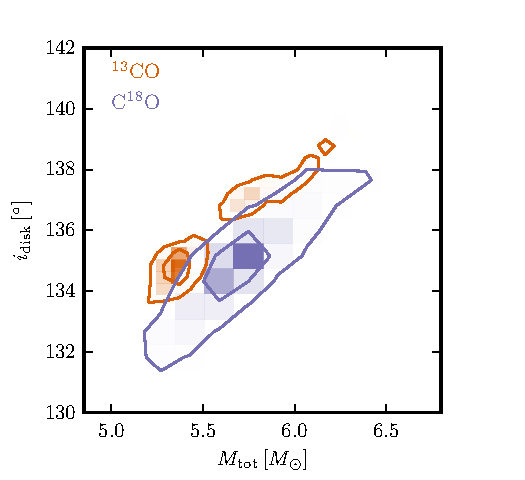
\includegraphics{posterior.pdf}
  \figcaption{Posterior distributions for the model parameters fit to the \thirteen\ and \eighteen\ data independently. \label{fig:posterior}}
  \end{center}
\end{figure}

The inferred parameter values corresponding to the measurements of each spectral line are summarized together in Table~\ref{table:components}.  A comparison of the data and the best-fit models (and associated residuals) is presented in the form of channel maps in Figures~\ref{fig:13co} and \ref{fig:c18o} for $^{13}$CO and C$^{18}$O, respectively.  While overall the models successfully reproduce the observed emission, there are some interesting systematic residuals.  We will return to a discussion of their potential origins in Section~\ref{sec:discussion}.  The inferred physical structures for each line are in mild disagreement, as might be expected for an over-simplified model based on data products that are sensitive to different regions of the disk.  Nevertheless, they both yield effectively identical constraints in the marginalized projection to the \{$M_\ast$, $i_d$\}-plane, as shown in Figure~\ref{fig:posterior}, that are of most relevance to our stated goals.  Again, that is because the kinematic structure of the line emission has very little dependence on the density and temperature parameters \citep[see][]{rosenfeld12a,czekala15a}.



\subsection{An Updated Model of the Stellar Orbits} \label{sec:orbit}

The discovery orbit of \gw\ by \cite{mathieu91}, with a period of
242 days, was based on a small subset of the same spectra used here,
covering slightly more than seven years. The present data set is six
times larger and extends the time coverage to nearly 35 years.
\cite{mathieu91} noted a drift in the residuals from their
spectroscopic orbit that they speculated could be due to a third
component, or perhaps an asymmetry in a massive circumbinary disk,
causing the reflex motion of the inner binary with a period exceeding
their time coverage. As our data set expanded over the years, our own
preliminary spectroscopic solutions for the 242-day orbit displayed an
increasingly clear periodic pattern in the residuals with a period of
about 11.5 years, strongly suggesting the presence of a third body in
the \gw\ system with a nearly circular orbit. Direct near-infrared
imaging by \cite{berger11} revealed the stellar nature of the third
component for the first time, and also resolved the inner binary.  Our
extended time coverage in radial velocities now enables us to derive a
robust spectroscopic orbit for the third star.

We used standard weighted non-linear least-squares techniques
\citep[e.g.,][]{press92} to solve for the elements of the inner and
outer Keplerian orbits simultaneously, assuming the inner binary acts
as a point mass in the outer orbit, and including the effects of light
travel time. Initial fits showed that a number of the measurements had
very large residuals, including instances of several consecutive
exposures over periods of a few days or weeks with residuals of the
same sign, possibly resulting from real phenomena such as flaring or
accretion events. A total of 23 such outliers were removed, and are
flagged in Table~\ref{tab:RVs}. The derived elements of the inner and
outer orbits are presented in Table~\ref{tab:elements}, along with
other properties derived from them. The residuals from our initial fit
indicated our formal velocity errors are slightly underestimated, so
for our final solution we have scaled them by a factor of 1.12 to
achieve a reduced $\chi^2$ of unity.


\begin{deluxetable}{lc}
\tablewidth{0pc}
\tablecaption{Spectroscopic orbital elements of \gw.\label{tab:elements}}
\tablehead{
\colhead{~~~~~~~~~~~~Parameter~~~~~~~~~~~~} & \colhead{Value}
}
\startdata
\multicolumn{2}{c}{Inner orbit} \\
\noalign{\vskip 1pt}
\noalign{\hrule}
\noalign{\vskip 3pt}
$P$ (days)\dotfill                        &    241.446~$\pm$~0.066\phn\phn \\
$\gamma$ (\kms)\dotfill                   &    +27.726~$\pm$~0.082\phn\phs \\
$K_{\rm A}$ (\kms)\dotfill                 &        3.54~$\pm$~0.11 \\
$e$\dotfill                               &      0.016~$\pm$~0.029 \\
$\omega$ (deg)\dotfill                    &        210~$\pm$~100 \\
$T_{\rm peri}$ (HJD$-$2,400,000)\dotfill   &      51861~$\pm$~67\phm{222} \\
\noalign{\vskip 2pt}
\noalign{\hrule}
\noalign{\vskip 2pt}
\multicolumn{2}{c}{Derived properties from inner orbit} \\
\noalign{\vskip 1pt}
\noalign{\hrule}
\noalign{\vskip 3pt}
$a_{\rm A} \sin i$ ($10^6$ \kms)\dotfill   &      11.76~$\pm$~0.36\phn \\
$f(M)$ ($M_{\sun}$)\dotfill                &    0.00111~$\pm$~0.00010 \\
$M_{\rm B} $($M_{\sun}$)\dotfill            &     0.1036~$\pm$~0.0031 \\
Time interval (days)\dotfill              &            12574 \\
Time interval (cycles)\dotfill            &             52.1 \\
\noalign{\vskip 2pt}
\noalign{\hrule}
\noalign{\vskip 2pt}
\multicolumn{2}{c}{Outer orbit} \\
\noalign{\vskip 1pt}
\noalign{\hrule}
\noalign{\vskip 3pt}
$P$ (days)\dotfill                        &       4187~$\pm$~42\phn\phn \\
$K_{\rm AB}$ (\kms)\dotfill                &       2.04~$\pm$~0.12 \\
$e$\dotfill                               &      0.061~$\pm$~0.058 \\
$\omega$ (deg)\dotfill                    &        276~$\pm$~48\phn \\
$T_{\rm peri}$ (HJD$-$2,400,000)\dotfill   &      53560~$\pm$~565\phn\phn \\
\noalign{\vskip 2pt}
\noalign{\hrule}
\noalign{\vskip 2pt}
\multicolumn{2}{c}{Derived properties from outer orbit} \\
\noalign{\vskip 1pt}
\noalign{\hrule}
\noalign{\vskip 3pt}
$a_{\rm AB} \sin i$ ($10^6$ \kms)\dotfill  &      117.0~$\pm$~6.7\phn\phn \\
$f(M)$ ($M_{\sun}$)\dotfill                &    0.00364~$\pm$~0.00062 \\
$M_{\rm C} $($M_{\sun}$)\dotfill            &     0.1539~$\pm$~0.0088 \\
Time interval (cycles)\dotfill            &             3.0 \\
\enddata
%\tablecomments{.}
\end{deluxetable}


The period of the inner orbit is consistent with that of
\cite{mathieu91}, and the eccentricity is insignificant, as was
also found by them. On the other hand, the velocity semi-amplitude of
our inner orbit, $K_{\rm A} = 3.54 \pm 0.11~\kms$, is significantly
smaller than theirs ($K_{\rm A} = 4.7 \pm 0.3~\kms$), but similar to
the one by \cite{fang14} ($K_{\rm A} = 3.41 \pm 0.17~\kms$).
Graphical representations of our observations and the inner and outer
orbit models as a function of orbital phase are shown in
Figure~\ref{fig:orbitin} and Figure~\ref{fig:orbitout}, respectively,
and a representation of the full motion as a function of time is seen
in Figure~\ref{fig:orbitboth}.


\begin{figure}
\epsscale{1.15}
\plotone{figorbit1.eps}
%
\figcaption[]{Radial-velocity measurements of \gw\ and best-fit model
  for the inner orbit, after subtracting the motion in the outer
  orbit. The dotted line in the top panel represents the
  center-of-mass velocity of the triple system. The bottom panel
  displays the residuals.\label{fig:orbitin}}
%
\end{figure}


\begin{figure}
\epsscale{1.15}
\plotone{figorbit2.eps}
%
\figcaption[]{Radial-velocity measurements of \gw\ and best-fit model
  for the outer orbit, after subtracting the motion in the inner
  orbit. The dotted line in the top panel represents the
  center-of-mass velocity of the triple system. The bottom panel
  displays the residuals.\label{fig:orbitout}}
%
\end{figure}


\begin{figure*}
\epsscale{1.15}
% \plotone{figout.eps}
\plotone{figout1.eps}
%
\figcaption[]{Radial-velocity measurements of \gw\ as a function of
  time, and best-fit model for the triple system. The dotted line
  represents the center-of-mass velocity.\label{fig:orbitboth}}
%
\end{figure*}

% RV variation of ~8-10 km/s coincides with an eclipse of ~0.6 mags in R, roughly gray. Might be caused by a knife-edge that has asymmetry wrt rotation axis (R-M effect).


\begin{deluxetable}{lr@{\,$\pm$\,}ll}
\tablecaption{Combined disk and RV constraints on component masses\label{table:components}}
\tablehead{\colhead{Parameter} & \multicolumn{2}{c}{Value} & \colhead{Unit}}
\startdata
$M_\mathrm{tot}$ & 5.50 & 0.20 & $M_\odot$ \\
$i_\mathrm{d}$ & 135 & 2 & degrees \\
$M_A$ & 4.40 & 0.18 & $M_\odot$ \\
$M_B$ & 0.42 & 0.02 & $M_\odot$ \\
$M_C$ & 0.68 & 0.05 & $M_\odot$ \\
\enddata
\end{deluxetable}

%
% \subsection{Expanded Catalog of Photometric Eclipses}
%
% % Presentation of photometry.
% % Catalog of eclipse dates
% % Discussion of possible occulter radius
%
% \begin{figure}[htb]
% \begin{center}
%   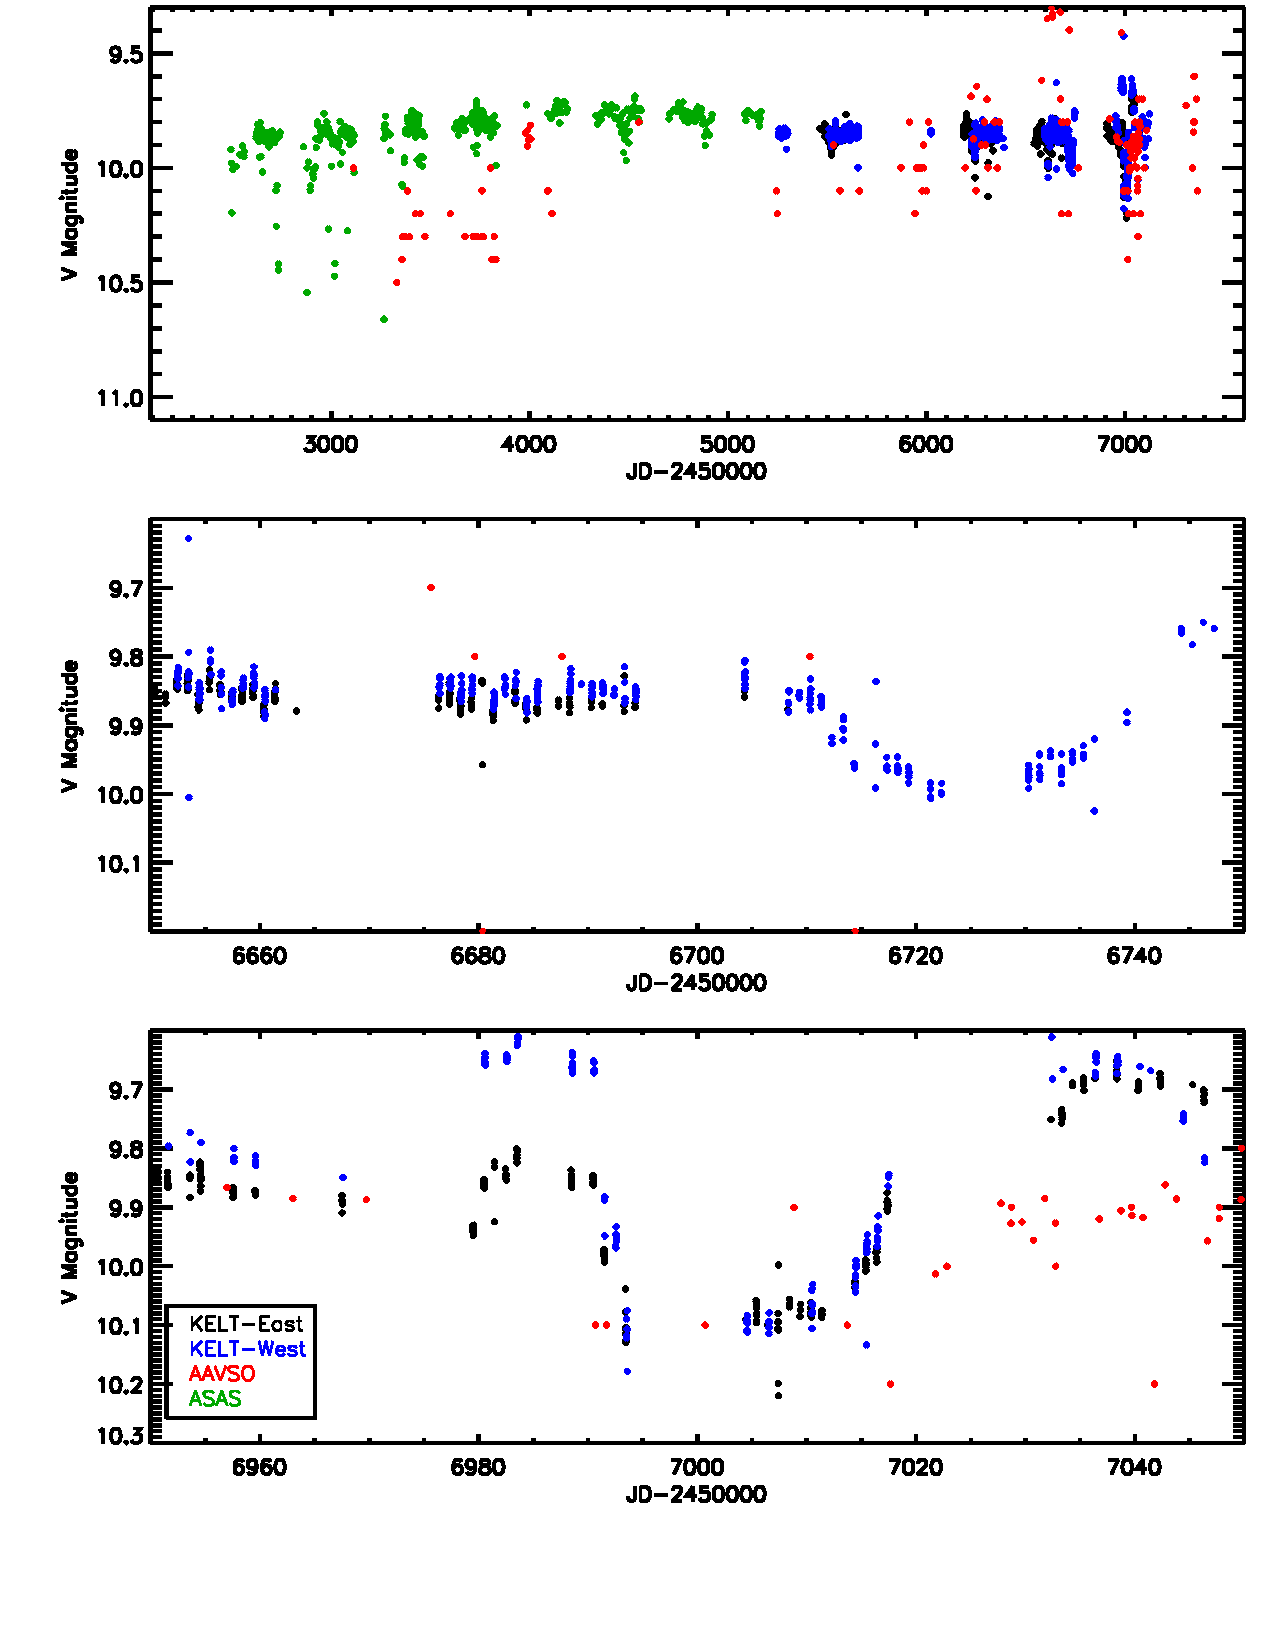
\includegraphics[height=0.5\textheight]{KELT_eclipses.pdf}
%   \figcaption{
%  KELT eclipses.
%   \label{fig:KELT}}
%   \end{center}
% \end{figure}
%
% Eclipses \citep{shevchenko92,shevchenko98}.
%
% Also see: http://arxiv.org/pdf/1608.07291v1.pdf
%
% \begin{deluxetable}{rrrrrl}
% % \tabletypesize{font size command}
% % \rotate
% % \tablewidth{dimen}
% % \tablenum{text}
% % \tablecolumns{6}
% \tablecaption{Photometric Eclipse Catalog\label{table:eclipses} \todo{NOTE: this eclipse data is only for reference when doing the RV fit to exclude outliers. NOT for publication until appropriate authors (Shevchenko et al.) have been contacted and their permission granted.}
% }
% \tablehead{\colhead{Eclipse Number} & \colhead{Start} & \colhead{End} & \colhead{Duration} & \colhead{Decrement} & \colhead{Telescope}\\
% & [JD] & [JD] & [days] & [mmag] & }
% \startdata
% \nodata & 2447043 & 2447056 & 13 & 600 & \nodata \\
% \nodata & 2447153 & 2447179 & 26 & 300 & \nodata \\
% \nodata & 2447418 & 2447435 & 17 & 450 & \nodata \\
% \nodata & 2447809 & 2447824 & 15 & 130 & \nodata \\
% \nodata & 2448137 & 2448162 & 25 & 300 & \nodata \\
% \nodata & 2448545 & 2448586 & 41 & 150 & \nodata \\
% \nodata & $\geq$2450399 & $\leq$2450414 & $\leq$15 & 300 & \nodata \\
% \nodata & 2452184 & $\geq$2452209 & $\geq$ 25 & 750 & \nodata \\
% \nodata & 2456710 & 2456744 & 34 & 130 & KELT \\
% \nodata & 2456989 & 2457030 & $\leq$41 & 220 & KELT \\ % Nov 28th, 2014
% \enddata
% \end{deluxetable}
%
% Figure from KELT, ASAS, and AAVSO.

\section{Discussion} \label{sec:discussion}

\todo{Discuss linear effect of unknown distance on mass.}

\subsection{The Evolutionary State of GW Ori A}
Pre-main sequence evolutionary models are commonly used to infer the mass and age of young stars using measurements of their photospheric properties. We now perform this exercise for the GW~Ori system and evaluate the consistency of the model predictions with our measured dynamical masses for each component.

Given our inability to detect secondary or tertiary spectral lines in our optical spectra, we assume that all of the visible light can be attributed to the photosphere of GW~Ori~A. We adopt the photospheric properties of GW~Ori~A as determined by \citet{fang14}, $T_\mathrm{eff} = 5500 \pm 200\,\mathrm{K}$ and $L = 48 \pm 10\,L_\odot$. These photospheric properties clearly place GW~Ori~A in a high mass region of the Hertzsprung Russell Diagram (see Figure~\ref{fig:PMS}, left). For example, the MIST models suggest that GW~Ori~A is at least $3 M_\odot$.

% List the models.
We evaluate the following pre-main sequence models: \citet{choi16} models, \citet{dotter08}, \citet{tognelli11}, and \citet{siess00}. We do not include the \citet{baraffe15} models because they do not include models with sufficiently massive stars. We evaluate the predictions of the evolutionary models in a Bayesian manner, following \citet{jorgensen05}. These models deliver (among other quantities) the photospheric properties as a function of stellar mass and age,
e.g., $T_\mathrm{eff}(M_\ast, \tau)$ and $L(M_\ast, \tau)$. The posterior probability distribution is then found by evaluating the consistency of the model predictions for a given \{$M_\ast$, $\tau$\} pair with the measured photospheric properties by \citet{fang14}, multiplied by any priors on  \{$M_\ast$, $\tau$\}, in which case we have none. The resulting posterior probability distributions are shown in Figure~\ref{fig:PMS} and are listed in Table~\ref{table:agreement}\footnote{Our code used to perform this analysis is available under an MIT open source license here: \url{https://github.com/iancze/ScottiePippen}}. In general, all four models make similar predictions about GW~Ori~A, $M_A \sim 3.9 \pm 3\,M_\odot$ and $\tau = 0.6 \pm 0.3\,$Myr. We assess the probability of consistency between the model-predicted mass and our dynamical mass by evaluating $p(M_\mathrm{model} = M_\mathrm{dyn}) = \int_0^\infty p_\mathrm{model}(M) \, p_\mathrm{dyn}(M) \, \mathrm{d}M$. For most models, the predicted stellar mass is significantly less than our measured dynamical mass, $M_A = 4.40 \pm 0.18\,M_\odot$, and is consistent only at the $2\sigma$ level. As mentioned by \citet{fang14}, GW~Ori~A is in an earlier evolutionary stage than Herbig Be stars, although it will eventually become one.

\begin{figure}[htb]
\begin{center}
  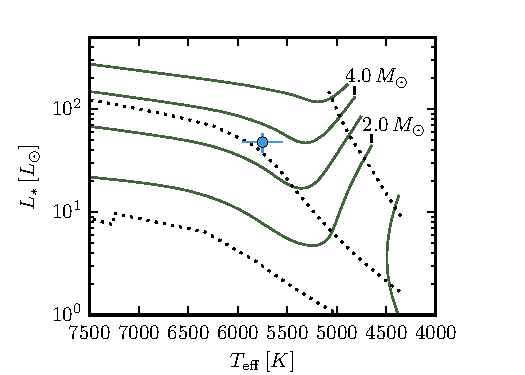
\includegraphics{tracks.pdf}
	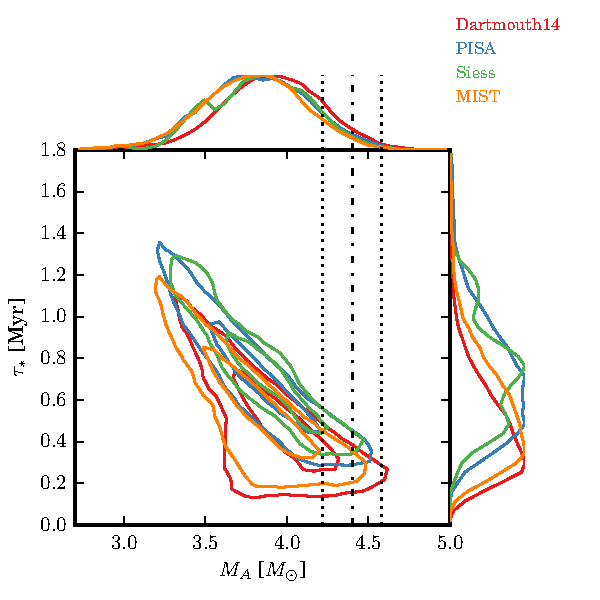
\includegraphics{agreement.pdf}
  \figcaption{\emph{left}: GW~Ori~A placed on the early Hertzsprung Russell diagram with the MIST evolutionary models. The mass tracks are 1 - 5 $M_\odot$ in intervals of 1 $M_\odot$, and the dotted lines denote isochrones for $0.1$, $1$, and $10$~Myr. Given the measured dynamical mass, GW~Ori~A is clearly underluminous. \emph{right}: The joint $M_A$ vs. $\tau$ posteriors with 1 and 2$\sigma$ contours, evaluated using a suite of pre-main sequence evolutionary model predictions. The top and right panels show the marginal mass and age posteriors, respectively. The mass inferred from the photospheric properties is in slight tension with our measured dynamical mass at the $1-2\sigma$ level.
  \label{fig:PMS}}
  \end{center}
\end{figure}

\begin{deluxetable}{lccc}
\tablecaption{Pre-main sequence model evaluation\label{table:agreement}.}
\tablehead{\colhead{Model} & \colhead{$M_A$ $[M_\odot]$} & \colhead{$\tau$ [Myr]} & \colhead{Consistency} }
\startdata
Dartmouth 14 & $3.96^{+0.30}_{-0.30}$ & $0.29^{+0.34}_{-0.05}$ & 44\% \\
PISA & $3.74^{+0.43}_{-0.18}$ & $0.74^{+0.20}_{-0.30}$ & 32\% \\
Seiss & $3.86^{+0.32}_{-0.32}$ & $0.79^{+0.12}_{-0.35}$ & 33\% \\
MIST & $3.86^{+0.27}_{-0.34}$ & $0.38^{+0.33}_{-0.11}$ & 27\%\\
\enddata
\tablecomments{Uncertainties are on the 68.3\% highest density interval. Agreement is the probability that the measurement of $M_A$ is consistent between the pre-main sequence model predictions from photospheric properties and our dynamical mass measurements.}
\end{deluxetable}

\paragraph{Constraints on GW~Ori~B and GW~Ori~C}
It was known early on that GW~Ori was at least a binary system \citet{mathieu91}--subsequent radial-velocity follow up revealed the presence of a long-period tertiary (D. Latham, \emph{private communication}). In 2011, \citet{berger11} used the IOTA/IONIC3 interferometer to reconstruct an H-band image of the GW~Ori system, revealing all three components. The mean H-band flux ratio (computed as the weighted mean of all measurements) is $f_B/f_A = 0.57 \pm 0.05$ and $f_C/f_A = 0.23 \pm 0.01$. In Figure~\ref{fig:evolution}, we plot the ratio of effective temperatures and the computed flux ratios in Bessell I band and 2MASS H band. Bessell I roughly corresponds to the reddest echelle orders of the TRES spectrograph that we used to search for companion spectral lines. These flux ratios are generally very small, and if correct, provide an explanation for why we were unable to detect secondary or tertiary spectral lines in our searches. This means that the excess H-band flux is likely due to the presence of a circumstellar disk or accretion signatures above the photospheric emission of these stars, assuming that all stars are the same age.

It is interesting to discuss the inferred dynamical masses of these components with the measured H-band fluxes of Berger and the non-detections of spectral lines in the visible. This seems to be consistent with the interpretation by \citet{berger11} about the likely disk contamination, otherwise the masses of A and B would be inferred to be near equal. To our knowledge there has been no radial velocity monitoring of GW~Ori in the infrared.

\begin{figure}[htb]
\begin{center}
  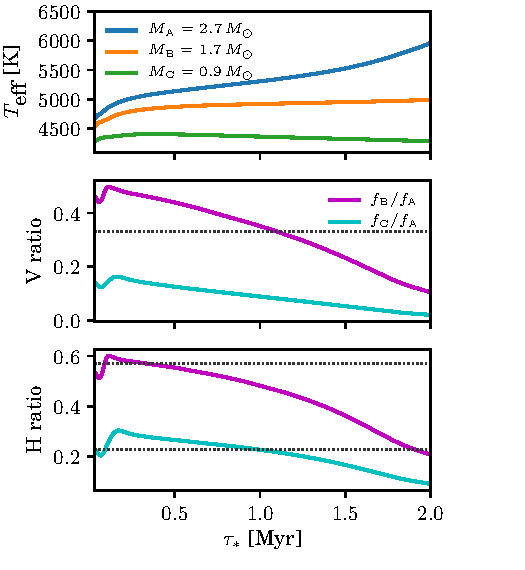
\includegraphics{evolution.pdf}
  \figcaption{Relative photospheric properties of the GW~Ori stellar components as a function of age, assuming they are coeval, predicted by the MIST pre-main sequence evolutionary models. \emph{top}: The cool effective temperature of GW~Ori~A indicates that it must be a very young star ($\tau < 5\,$Myr). The nominal age of GW Ori as predicted by the MIST models is labeled as a vertical dashed line. \emph{middle and bottom}: the predicted flux contrasts in Bessell I band and 2MASS H, respectively.
  \label{fig:evolution}}
  \end{center}
\end{figure}


\subsection{GW Ori as a triple system}
It is now clear that GW Ori is a massive triple star system ($M_\mathrm{tot} = 5.5\,M_\odot$), hosting a massive \citep[$M_\mathrm{disk} \sim 1.5\,M_\odot$;][]{mathieu95} and large ($r_c \sim 1000\,\mathrm{AU}$) disk. Given the observed composite spectrum and inferred mass ratios (Sec 4) it is also likely that the system is very young, making GW Ori an extremely interesting system to study in the context of star and planet theories about formation, migration, and stability.


\textbf{How did the various components form?}
Fragmentation can be due to cooling or accretion. Highly variable accretion can force disks up to the fragmentation threshold, where binarity is a frequent outcome. Consensus that GI-formed objects will become brown dwarfs or stellar binary companions \citep{kratter10}, due to moderate disk temperatures and active accretion, which will grow these GI formed objects to higher masses.

\citep{stamatellos09} BD formed in massive disks, but disks should be short lived. (Prediction for GW Ori lifetime?) Clearly disks are older than a few thousand years (their prediction). Predict lower mass objects are ejected by dynamical interactions. Disk fragmentation is a robust mechanism for brown dwarf formation. Again, most objects formed in disk grow to brown dwarf or hydrogen burning masses.

\citep{forgan13} objects that form via GI, 90\% are above deuterium burning limits. Population synthesis model. GI then tidal downsizing is not principal mode of planet formation, but is primary means of forming brown dwarfs and low mass stars at large $a$.

\citep{offner10}.
Turbulent fragmentation is dominant channel for binary formation for \emph{low mass} stars. Is disk accretion ever so violent that it induces disk fragmentation? The fact (assumption?) that everything is coplanar and low eccentricity are expected from fragmentation from a single disk. Conclude that binaries are formed via turbulent core fragmentation (not disk). Disks are not massive enough to have gravitational instability in the disk. \citet{offner10} cite Howe \& Clarke 2009 for a review of observations.

\citet{tokovinin97} finds that the distribution of mutual inclinations of the orbits in triple systems is inconsistent both with complete alignment of the inner and outer orbits, but also with independent inclinations of the two orbits.  However, we should note that this is for a population of much older systems, in which significant dynamical evolution could have occurred, particularly for the shorter-period systems.  The fact that GW Ori appears to have roughly-aligned, circular inner and outer orbits (!! does it?  to be confirmed) is suggestive of formation of one or both companions from the massive disk surrounding the system.  (Wild speculation here.)

Speculation from \citet{berger11} about whether the stellar system is actual stable.


\textbf{Is the disk stable today?}
\textbf{What does this mean for future observations: scattered light, high res, etc.}
Given the large disk mass and the massive components, it is natural to question whether these components formed from disk fragmentation due to gravitational instability, and whether the disk is itself Toomre stable today. Disks most likely to be stable are young and $M_d/M_\ast > 0.1$. Develop spiral arms. Thermodynamics drive instabilities, which may fragment into bound companions. Cold outer disk (free of MHD, usually) is the most likely to become gravitationally unstable. \todo{Estimate Toomre Q parameters from Kratter review, eqn 3. Seems like the disk is definitely Q unstable.} \citet{kratter16}.

Discussion of GW~Ori disk mass in context of \citet{andrews13}. Note Eisner 12, Sheehan and Eisner 14 discuss high disk masses in Taurus class I (younger sources).

Mann 15 also suggests young sources have more massive disks. NGC 2024.

Shepherd 01, 04 rotating disk around B star.



\textbf{Eric}: Some notes from Eric from reading literature on what is known about triple systems.  Is this extreme?

While the ratio between the outer orbital period and the inner orbital period is smaller than in many hierarchical systems, it is not an outlier among triple systems.  In a detailed analysis of higher-order multiple systems, \citet{tokovinin97} found that the ratio $P_\mathrm{long} / P_{\rm short}$ in almost all systems was greater than 10, presumably reflecting which orbits are stable.  In GW Ori, this ratio is 16.

(Tokovinin has an updated catalog on his website with about twice as many systems as in the CDS version from this paper, but it would be non-trivial to figure out how to remake the above plot.  Not sure it's necessary.)

Among late B star primaries (which GW Ori A will be on the main sequence), 13\% of systems have multiplicity of three or higher \citep{eggleton08}; this fraction is roughly constant across spectral types B--G.


Bate 2012 on his big fragmentation simulation: ``In particular, despite the fact that no objects form closer than $\approx 10$ au from each other, at the end of the calculation there exist 21 binary systems and one triple system with separations $<10$ au.''

In his simulations, of the triples that form, the orbits are misaligned with each other (though three are $\leq 6$ degrees, and 8 out of 9 are $\leq 36$ degrees).

Bate:  ``Observations also indicate that eccentricities $e < 0.1$ are rare for periods greater than $\approx$ 100 d (separations $\gtrsim$ 1 au). Raghavan et al. (2010) find no binaries with $e < 0.1$ and orbital periods greater than 100 d, though they do find that the outer orbits of two triples and one quadruple have $e < 0.1$. Duquennoy \& Mayor (1991) and Raghavan et al. (2010) also find that the upper-eccentricity envelope is dominated by components of triple systems, possibly due to the action of the Kozai mechanism (Kozai 1962).''

Important for us to see what constraints we have on eccentricity of the orbits.



\subsection{The inner ~100 \,AU of the GW~Ori system} \label{sec:inner disk}

CO sub-mm excess.

Najita's blended fundamental emission peaks \citep{najita03}, while \citet{bast11} suggest that these might actually be the blended profiles of emission originating from physically distinct regions. In this case, perhaps individual circumstellar disks around the A and B stars. Or, the CO fundamental emission is consistent with with radius at the inner edge of the circumtriple disk, cleared by the C component. The tertiary star makes a complicated accretion flow than that studied for other well-known binaries \citep[e.g., DQ~Tau;]{artymowicz94,mathieu97}.

Photometric eclipses. This complicated tertiary flow may also contribute to photometric eclipses seen in the optical. Not all are periodic, but some regularity with period? Can we record what orbital phases they occur at? Maybe there is some correlation with A and B.

Ansdell dippers

Stellar orbits

Diagram showing the as-measured stellar orbits.

Is the tertiary in the disk? What is the effect of the tertiary orbit on the disk.

\citep{offner16}. Outflows (jets) and protostellar spins are misaligned. Does this match our central excess?

\section{Summary and Conclusions} \label{sec:summary}

\acknowledgments
IC acknowledges support from the Smithsonian Institution for the production of this manuscript. IC acknowledges helpful conversations with Maxwell Moe about GW Ori and related systems.  SA acknowledges the very helpful support provided by the NRAO Student Observing Support program related to the early development of this project.  This paper makes use of the following ALMA data: XX  ALMA is a partnership of ESO (representing its member states), NSF (USA), and NINS (Japan), together with NRC (Canada) and NSC and ASIAA (Taiwan), in cooperation with the Republic of Chile.  The Joint ALMA Observatory is operated by ESO, AUI/NRAO, and NAOJ.  This research made extensive use of the Julia programming language \citep{julia12} and Astropy \citep{astropy13}.

\bibliographystyle{aasjournal.bst}
\bibliography{GWOri.bib}

\end{document}
